% Options for packages loaded elsewhere
\PassOptionsToPackage{unicode}{hyperref}
\PassOptionsToPackage{hyphens}{url}
%
\documentclass[
  english,
  man,floatsintext]{apa6}
\usepackage{amsmath,amssymb}
\usepackage{lmodern}
\usepackage{iftex}
\ifPDFTeX
  \usepackage[T1]{fontenc}
  \usepackage[utf8]{inputenc}
  \usepackage{textcomp} % provide euro and other symbols
\else % if luatex or xetex
  \usepackage{unicode-math}
  \defaultfontfeatures{Scale=MatchLowercase}
  \defaultfontfeatures[\rmfamily]{Ligatures=TeX,Scale=1}
\fi
% Use upquote if available, for straight quotes in verbatim environments
\IfFileExists{upquote.sty}{\usepackage{upquote}}{}
\IfFileExists{microtype.sty}{% use microtype if available
  \usepackage[]{microtype}
  \UseMicrotypeSet[protrusion]{basicmath} % disable protrusion for tt fonts
}{}
\makeatletter
\@ifundefined{KOMAClassName}{% if non-KOMA class
  \IfFileExists{parskip.sty}{%
    \usepackage{parskip}
  }{% else
    \setlength{\parindent}{0pt}
    \setlength{\parskip}{6pt plus 2pt minus 1pt}}
}{% if KOMA class
  \KOMAoptions{parskip=half}}
\makeatother
\usepackage{xcolor}
\IfFileExists{xurl.sty}{\usepackage{xurl}}{} % add URL line breaks if available
\IfFileExists{bookmark.sty}{\usepackage{bookmark}}{\usepackage{hyperref}}
\hypersetup{
  pdftitle={AI-based recognition of momentary subjective affect experience from natural speech},
  pdfauthor={Timo K. Koch1,2, Gabriella M. Harari3, Ramona Schoedel2,4, Zachariah Marrero5, Florian Bemmann6, Samuel D. Gosling5, Markus Buehner2, \& Clemens Stachl1},
  pdflang={en-EN},
  pdfkeywords={Affect, Speech, Voice, Machine Learning, Mobile Sensing},
  hidelinks,
  pdfcreator={LaTeX via pandoc}}
\urlstyle{same} % disable monospaced font for URLs
\usepackage{graphicx}
\makeatletter
\def\maxwidth{\ifdim\Gin@nat@width>\linewidth\linewidth\else\Gin@nat@width\fi}
\def\maxheight{\ifdim\Gin@nat@height>\textheight\textheight\else\Gin@nat@height\fi}
\makeatother
% Scale images if necessary, so that they will not overflow the page
% margins by default, and it is still possible to overwrite the defaults
% using explicit options in \includegraphics[width, height, ...]{}
\setkeys{Gin}{width=\maxwidth,height=\maxheight,keepaspectratio}
% Set default figure placement to htbp
\makeatletter
\def\fps@figure{htbp}
\makeatother
\setlength{\emergencystretch}{3em} % prevent overfull lines
\providecommand{\tightlist}{%
  \setlength{\itemsep}{0pt}\setlength{\parskip}{0pt}}
\setcounter{secnumdepth}{-\maxdimen} % remove section numbering
% Make \paragraph and \subparagraph free-standing
\ifx\paragraph\undefined\else
  \let\oldparagraph\paragraph
  \renewcommand{\paragraph}[1]{\oldparagraph{#1}\mbox{}}
\fi
\ifx\subparagraph\undefined\else
  \let\oldsubparagraph\subparagraph
  \renewcommand{\subparagraph}[1]{\oldsubparagraph{#1}\mbox{}}
\fi
% Manuscript styling
\usepackage{upgreek}
\captionsetup{font=singlespacing,justification=justified}

% Table formatting
\usepackage{longtable}
\usepackage{lscape}
% \usepackage[counterclockwise]{rotating}   % Landscape page setup for large tables
\usepackage{multirow}		% Table styling
\usepackage{tabularx}		% Control Column width
\usepackage[flushleft]{threeparttable}	% Allows for three part tables with a specified notes section
\usepackage{threeparttablex}            % Lets threeparttable work with longtable

% Create new environments so endfloat can handle them
% \newenvironment{ltable}
%   {\begin{landscape}\centering\begin{threeparttable}}
%   {\end{threeparttable}\end{landscape}}
\newenvironment{lltable}{\begin{landscape}\centering\begin{ThreePartTable}}{\end{ThreePartTable}\end{landscape}}

% Enables adjusting longtable caption width to table width
% Solution found at http://golatex.de/longtable-mit-caption-so-breit-wie-die-tabelle-t15767.html
\makeatletter
\newcommand\LastLTentrywidth{1em}
\newlength\longtablewidth
\setlength{\longtablewidth}{1in}
\newcommand{\getlongtablewidth}{\begingroup \ifcsname LT@\roman{LT@tables}\endcsname \global\longtablewidth=0pt \renewcommand{\LT@entry}[2]{\global\advance\longtablewidth by ##2\relax\gdef\LastLTentrywidth{##2}}\@nameuse{LT@\roman{LT@tables}} \fi \endgroup}

% \setlength{\parindent}{0.5in}
% \setlength{\parskip}{0pt plus 0pt minus 0pt}

% Overwrite redefinition of paragraph and subparagraph by the default LaTeX template
% See https://github.com/crsh/papaja/issues/292
\makeatletter
\renewcommand{\paragraph}{\@startsection{paragraph}{4}{\parindent}%
  {0\baselineskip \@plus 0.2ex \@minus 0.2ex}%
  {-1em}%
  {\normalfont\normalsize\bfseries\itshape\typesectitle}}

\renewcommand{\subparagraph}[1]{\@startsection{subparagraph}{5}{1em}%
  {0\baselineskip \@plus 0.2ex \@minus 0.2ex}%
  {-\z@\relax}%
  {\normalfont\normalsize\itshape\hspace{\parindent}{#1}\textit{\addperi}}{\relax}}
\makeatother

\makeatletter
\usepackage{etoolbox}
\patchcmd{\maketitle}
  {\section{\normalfont\normalsize\abstractname}}
  {\section*{\normalfont\normalsize\abstractname}}
  {}{\typeout{Failed to patch abstract.}}
\patchcmd{\maketitle}
  {\section{\protect\normalfont{\@title}}}
  {\section*{\protect\normalfont{\@title}}}
  {}{\typeout{Failed to patch title.}}
\makeatother

\usepackage{xpatch}
\makeatletter
\xapptocmd\appendix
  {\xapptocmd\section
    {\addcontentsline{toc}{section}{\appendixname\ifoneappendix\else~\theappendix\fi\\: #1}}
    {}{\InnerPatchFailed}%
  }
{}{\PatchFailed}
\keywords{Affect, Speech, Voice, Machine Learning, Mobile Sensing\newline\indent Word count: 5505}
\usepackage{csquotes}
\ifXeTeX
  % Load polyglossia as late as possible: uses bidi with RTL langages (e.g. Hebrew, Arabic)
  \usepackage{polyglossia}
  \setmainlanguage[]{english}
\else
  \usepackage[main=english]{babel}
% get rid of language-specific shorthands (see #6817):
\let\LanguageShortHands\languageshorthands
\def\languageshorthands#1{}
\fi
\ifLuaTeX
  \usepackage{selnolig}  % disable illegal ligatures
\fi
\newlength{\cslhangindent}
\setlength{\cslhangindent}{1.5em}
\newlength{\csllabelwidth}
\setlength{\csllabelwidth}{3em}
\newenvironment{CSLReferences}[2] % #1 hanging-ident, #2 entry spacing
 {% don't indent paragraphs
  \setlength{\parindent}{0pt}
  % turn on hanging indent if param 1 is 1
  \ifodd #1 \everypar{\setlength{\hangindent}{\cslhangindent}}\ignorespaces\fi
  % set entry spacing
  \ifnum #2 > 0
  \setlength{\parskip}{#2\baselineskip}
  \fi
 }%
 {}
\usepackage{calc}
\newcommand{\CSLBlock}[1]{#1\hfill\break}
\newcommand{\CSLLeftMargin}[1]{\parbox[t]{\csllabelwidth}{#1}}
\newcommand{\CSLRightInline}[1]{\parbox[t]{\linewidth - \csllabelwidth}{#1}\break}
\newcommand{\CSLIndent}[1]{\hspace{\cslhangindent}#1}

\title{AI-based recognition of momentary subjective affect experience from natural speech}
\author{Timo K. Koch\textsuperscript{1,2}, Gabriella M. Harari\textsuperscript{3}, Ramona Schoedel\textsuperscript{2,4}, Zachariah Marrero\textsuperscript{5}, Florian Bemmann\textsuperscript{6}, Samuel D. Gosling\textsuperscript{5}, Markus Buehner\textsuperscript{2}, \& Clemens Stachl\textsuperscript{1}}
\date{}


\shorttitle{Subjective Affect Experience in Natural Speech}

\authornote{

Conflict of interest: none
Acknowledgements: We thank Peter Ehrich and Dominik Heinrich for their support with the technical implementation of the on-device voice feature extraction and the ZPID for the support with data collection for study 1. Thank you Sumer Vaid for the technical support with the set up of the environment for the analyses of study 2. This project was supported by the Swiss National Science Foundation (SNSF) under project number 215303 and a scholarship of the German Academic Scholarship Foundation awarded to the first author.
All materials are available in the project's repository on the Open Science Framework (OSF): \url{https://osf.io/a5db8/}

The authors made the following contributions. Timo K. Koch: Conceptualization, Formal Analysis, Writing - Original Draft Preparation, Writing - Review \& Editing; Gabriella M. Harari: Writing - Review \& Editing, Supervision; Ramona Schoedel: Conceptualization, Writing - Review \& Editing; Zachariah Marrero: Data curation; Florian Bemmann: Software; Samuel D. Gosling: Resources; Markus Buehner: Resources; Clemens Stachl: Writing - Review \& Editing, Supervision.

Correspondence concerning this article should be addressed to Timo K. Koch, Postal address. E-mail: \href{mailto:timo.koch@unisg.ch}{\nolinkurl{timo.koch@unisg.ch}}

}

\affiliation{\vspace{0.5cm}\textsuperscript{1} Institute of Behavioral Science and Technology, University of St.~Gallen\\\textsuperscript{2} Department of Psychology, Ludwig-Maximilians-Universität München\\\textsuperscript{3} Stanford University\\\textsuperscript{4} Charlotte Fresensius Hochschule, University of Psychology\\\textsuperscript{5} University of Texas\\\textsuperscript{6} Media Informatics Group, Ludwig-Maximilians-Universität München}

\abstract{%
Advances in the area of artificial intelligence (AI) and the ubiquity of speech data, for example from voice assistants, have created numerous commercial products that claim to be able to automatically recognize emotions from human voice. However, the employed algorithms have often been trained solely on enacted or labelled speech samples from artificial lab settings representing affect \emph{expression} and are used to infer everyday subjective affect \emph{experience}. In the present work, we investigate if machine learning algorithms can truly recognize subjective affect momentary experience from speech samples collected in the wild. In two studies, we extract acoustic voice parameters and state-of-the-art word embeddings from 24766 speech samples with corresponding experience-sampled self-reports on momentary affect experience from 997 participants collected using off-the-shelf smartphones. While voice acoustics provide limited predictive information of subjective affective arousal, speech content is much more predictive. From voice cues, the fundamental frequency, spectral flux, and loudness revealed most affective information. Further, experimental and explorative findings suggest that emotional speech content does not affect predictions from voice acoustics (i.e., what someone talks about does not affect how well emotions can be inferred from voice cues alone). We discuss implications for the algorithmic monitoring of affect experience from speech in everyday life.
}



\begin{document}
\maketitle

\hypertarget{introduction}{%
\section{Introduction}\label{introduction}}

Research findings on the algorithmic recognition of affective states and related affective disorders from speech offer promising applications, for instance in health care, human-machine interaction, education, and marketing (Hildebrand et al., 2020; Milling, Pokorny, Bartl-Pokorny, \& Schuller, 2022). The advances in algorithmic affect recognition from speech leveraging AI and the ubiquity of available speech data due to the rise of voice assistants, for example Amazon's Alexa and Apple's Siri, have created an increasing commercial interest in the field. Here, tech companies aim to leverage speech data to, for instance, recognize what momentary affect their customers experience in order to develop personalized user interfaces or make product recommendations (Knight, 2016; Mandell, 2020; Vlahos, 2019). Most of the prediction models used in research and in the corresponding commercial tools are trained on enacted or labelled speech samples from artificial lab settings that represent emotion \emph{expressions}. However, those algorithms are often deployed to detect people's subjective affect \emph{experience} in everyday life. Further, many of the commercial algorithms are not transparent with regard to how well their predictions work and how (biased) predictions are being made. These issues raise questions regarding the reliability of emotion-detecting speech technology and the protection of user privacy in setting where speech data can be analyzed, for example, when using voice assistants. The present work investigates the algorithmic recognition of subjective self-reported momentary affect \emph{experience} from speech samples collected with smartphones in everyday life.

\hypertarget{predicting-affect-expressions-versus-subjective-affect-experience-from-voice-cues}{%
\subsection{Predicting affect expressions versus subjective affect experience from voice cues}\label{predicting-affect-expressions-versus-subjective-affect-experience-from-voice-cues}}

Prior research has reported on successfully predicting affective states (e.g., emotions) from a range of speech data, such as labelled TV clips (Grimm, Kroschel, \& Narayanan, 2008), phone calls, and enacted speech samples from the lab (Bänziger, Mortillaro, \& Scherer, 2012; Burkhardt, Paeschke, Rolfes, Sendlmeier, \& Weiss, 2005; Schuller, 2018; Vogt, André, \& Wagner, 2008). They report on impressive prediction performances for the automatic recognition of emotions (i.e., correlations between true scores and predicted scores of up to .81 for arousal and .68 for valence predictions) (Weninger, Eyben, Schuller, Mortillaro, \& Scherer, 2013). However, one has to keep in mind that in those works the enacted target emotion or the rater labels serve as ground truth. Thereby, these works predict affect \emph{expression}, which is considered easier to algorithmically recognize than real-life \emph{experienced} affect (Vogt, André, \& Wagner, 2008). There is a fundamental difference between what affect we express and what affect we actually experience, even though there is an overlap to a varying degree. Affect \emph{expression} represents the emotional expressive behavior based on our internal affect \emph{experience}. However, ``feeling is not always revealing,'' i.e., one does not necessarily express what one experiences affectively or might even express something completely different (J. A. J. Gross \& John, 1997; J. J. Gross, John, \& Richards, 2000). Furthermore, the way one expresses affect might be perceived and interpreted differently. Figure \ref{fig:experiencevsexpression} depicts this distinction. Moreover, the prediction performance varies greatly across studies due to a varying choice of emotion targets (i.e., discrete emotion versus core affect), conceptualizations of affect (e.g., short-termed elicited emotions versus moods), and employed algorithms (e.g., supervised versus unsupervised machine learning).

\begin{figure}

{\centering 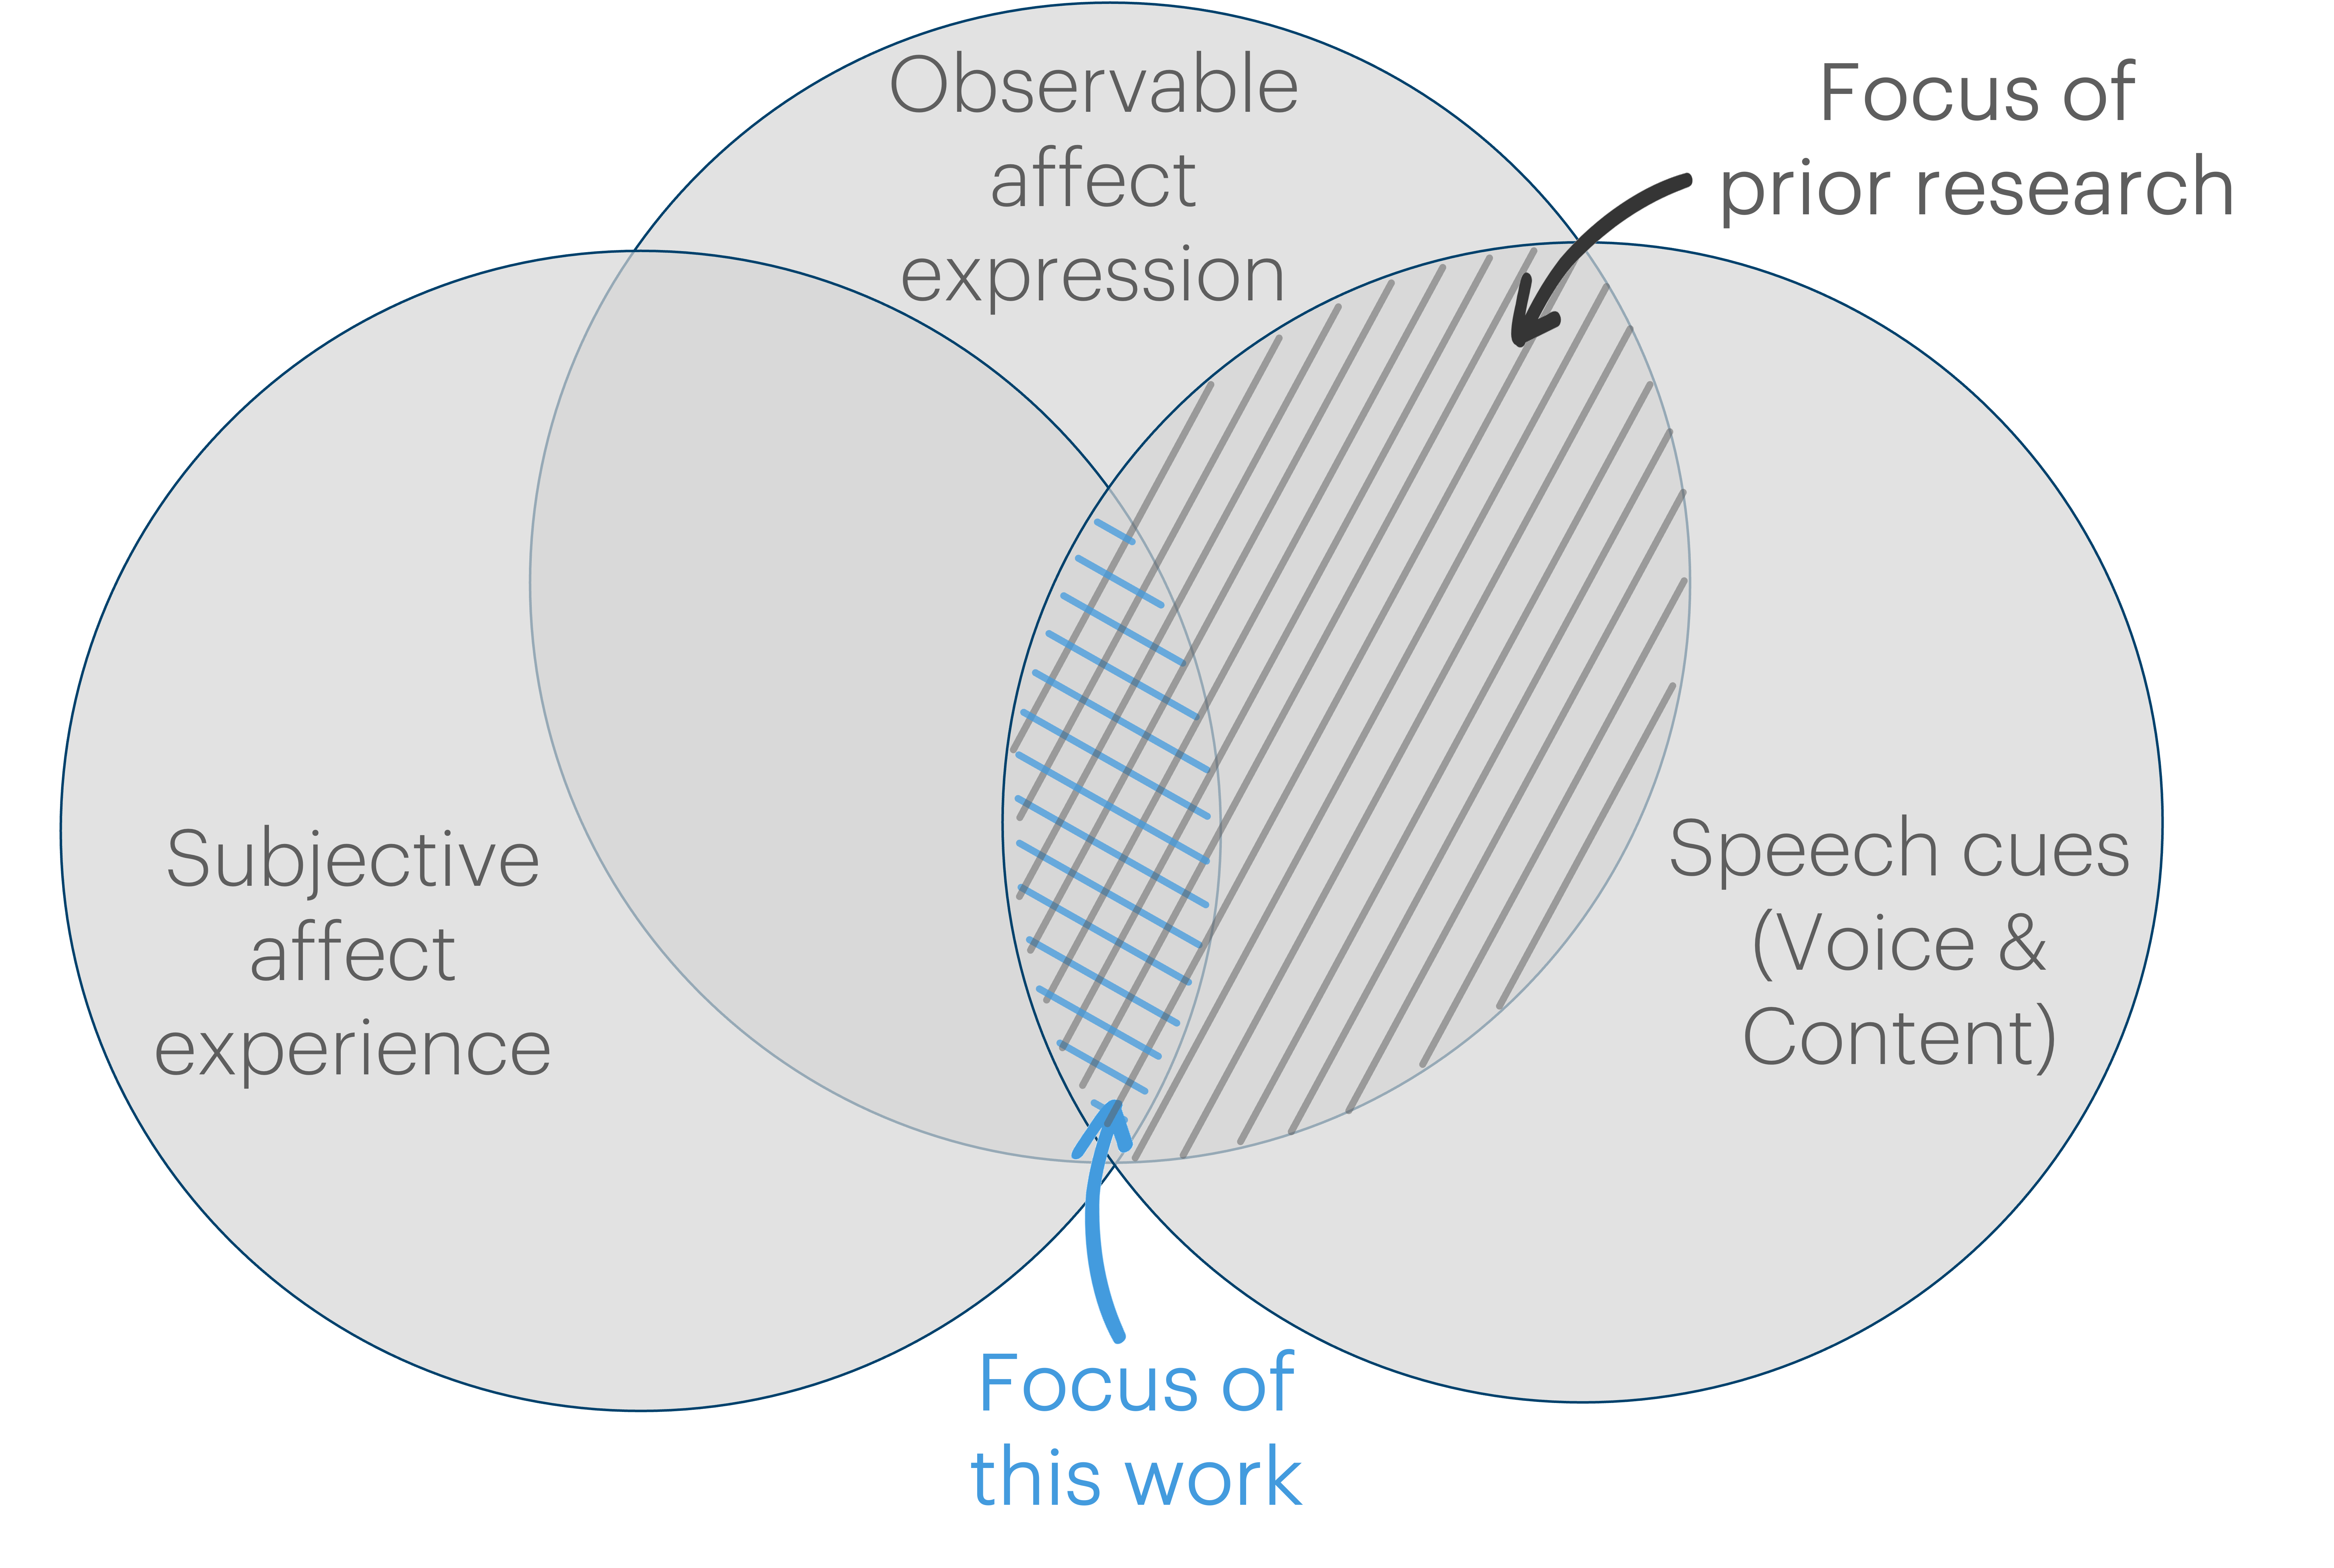
\includegraphics[width=0.75\linewidth]{../figures/experience_vs_expression} 

}

\caption[Feature importance]{The difference of subjective affect experience and observable affect expression and how they overlap with speech cues.}\label{fig:experiencevsexpression}
\end{figure}

Due to the challenge of obtaining speech data with corresponding affect labels in-vivo, most prior research on affect recognition from speech has used actors or labelled samples. This comes with a set of downsides, such as actors potentially overacting and the ambiguity of ground truth due to the subjective nature of labeling (Batliner et al., 2011; Schuller, 2018; Wilting, Krahmer, \& Swerts, 2006). As a consequence, studies investigating predictions of subjective affect experience from speech are rare. Recent works have collected everyday speech samples using the Electronically Activated Recorder (EAR) (Mehl, 2017). Hereby, speech data can be collected over a period of time which allows researchers to not only investigate between-person differences in affect (i.e., is this person sad?), but also assess within-person fluctuations (i.e., is this person sadder than other days?) (Huang \& Epps, 2018; Sun, Schwartz, Son, Kern, \& Vazire, 2020; Weidman et al., 2020). Using the EAR, however, can be privacy invasive since potentially non-consenting persons may be recorded, too. Moreover, handling the EAR recorders and transmitting the collected data can be tedious for participants and researchers.
Here, off-the-shelf smartphones represent a useful platform to collect experience samples on momentary affect experience over time and make corresponding speech records using the build-in microphone (Carlier et al., 2022; Sun, Schwartz, Son, Kern, \& Vazire, 2020; Weidman et al., 2020).

\hypertarget{prosody-content-interactions-in-affect-recognition-from-speech}{%
\subsection{Prosody-content interactions in affect recognition from speech}\label{prosody-content-interactions-in-affect-recognition-from-speech}}

Prior research has shown that prosody and the lexical content of the produced words (semantics) work together when transmitting affective information through speech (Ben-David, Multani, Shakuf, Rudzicz, \& van Lieshout, 2016). Moreover, some studies even suggest that there is a prosodic (i.e., from voice cues) dominance in the perception of affect based on lab experiments (Ben-David, Multani, Shakuf, Rudzicz, \& van Lieshout, 2016; \textbf{linProsodyDominatesSemantics2020?}), but not (yet) using speech data from the wild (Schwartz \& Pell, 2012). Moreover, while this research field had focused on the interplay of prosody and semantics in the recognition of affect by human raters, there are, to our knowledge, no studies on prosody-content interactions in algorithmic affect detection. Hence, it is currently unclear if what users talk about (i.e., the emotional content) has an effect on voice acoustics that impact automated affect recognition. In an applied setting, for example, the question is if an algorithm could recognize affective states regardless of what the person talks about, may it be a mundane topic, such as the weather or ordering pizza, or does one need to talk about an emotionally loaded topic (e.g., meeting a loved one).

\hypertarget{the-ambiguous-sound-of-expressed-emotional-prosody}{%
\subsection{The ambiguous sound of expressed emotional prosody}\label{the-ambiguous-sound-of-expressed-emotional-prosody}}

For AI models to decipher the nuanced relationship between acoustic prosody and affective states, they need to learn from the complex interplay of acoustic features. A recent review by Larrouy-Maestri et al. (Larrouy-Maestri, Poeppel, \& Pell, 2024) highlights how pitch, volume, speech rate, and voice quality, or timbre, serve as central cues in conveying emotions. For instance, higher pitch and faster speech rates are generally associated with excitement or stress, indicating a universal trend across languages and cultures. However, (van Rijn \& Larrouy-Maestri, 2023) demonstrate significant variability in the mapping of emotions to speech prosody across different cultures and languages. This variability underscores the challenges faced by AI in affect recognition, emphasizing that while certain prosodic features might be universally recognized, their interpretation can vary dramatically between individuals and cultural contexts. These findings underscore the importance of incorporating a diverse array of contexts, such as culture, to enhance the accuracy of AI tools.

Furthermore, the works of Banse and Scherer (Banse \& Scherer, 1996) and Scherer (Scherer, 2003) contribute to this discourse by exploring the reliability, specificity, and generalizability of these affect-voice mappings. They show that while there is a degree of consistency in how emotions are expressed and perceived through prosody, significant variability exists. This is echoed in Juslin \& Laukka's (2003) comparison of vocal expression and music performance, suggesting that different channels might employ the same code in communicating emotions, yet the effectiveness and interpretation of these codes can vary. However, again, all those findings are based on data, for example, from actors representing affect expressions and it remains unclear if they also transfer to subjective affect experience.

The present work leverages methodological advances in the area of smartphone-based data collection methods to investigate the prediction of subjective momentary affect experience from speech. In two large-scale studies, we train cross-validated machine learning models on acoustic voice cues and state-of-the-art word embeddings from speech samples collected in the wild. In those models, we experimentally and exploratively investigate the effects of the emotionality of speech's content on algorithmic affect recognition from voice acoustics. Moreover, we investigate which voice cues are carry the most affective information. Thereby, we aim to inform potential applications and promises in automatic affect recognition from speech signals and advise the discussion on the protection of user privacy rights.

\newpage

\hypertarget{method}{%
\section{Method}\label{method}}

\hypertarget{study-1-data-collection}{%
\subsection{Study 1: Data collection}\label{study-1-data-collection}}

Data collection for study 1 was part of a large six-month panel study (from May until November 2020) using the \emph{PhoneStudy} research app at Ludwig-Maximilian-Universität München (Schoedel \& Oldemeier, 2020). Data collection was approved by the responsible IRB board. The study comprised two two-week experience sampling phases (July 27, 2020, to August 9,2020; September 21, 2020, to October 4, 2020) during which participants received two to four short questionnaires per day. Here, self-reported valence and arousal were assessed in two separate items on six-point Likert scales among other psychological properties as part of an experience sampling procedure.

The last experience sampling questionnaire of each day included an additional instruction, where participants were asked to read out a series of predefined emotional sentences while making an audio recording of their voice. The sentences presented to the participants are based on a set of validated German neutral and affective sentences (Defren et al., 2018) and differ in their emotional content: positive (e.g., ``My team won yesterday.''), negative (e.g., ``Nobody is interested in my life.''), and neutral (e.g., ``The plate is on the round table.''). These three emotional categories are presented consecutively in each audio logging task. The order of the categories was randomized per experience sampling questionnaire. For each emotional content category, three sentences were randomly drawn from respective sets of sentences in the database. The use and experimental manipulation of these emotional semantic categories allowed us to control for the content spoken by our participants and at the same time enabled us to conduct a privacy-friendly study. The audio recording was started by the participants via a button on the screen. Participants could stop the recording manually after a minimum of four seconds. Alternatively, the recording was stopped automatically after twelve seconds. We chose these lower- and upper-time thresholds because this is the minimum and maximum time required to read out the three sentences per condition.
Once the audio record had been completed, we used the widely adopted \emph{OpenSMILE} open-source algorithm (Eyben, Wöllmer, \& Schuller, 2010) to automatically extract acoustic features directly on the participant's device. Here, we used the extended Geneva Minimalistic Acoustic Parameters Set (eGeMAPS) that is comprised of 88 acoustic features (Eyben et al., 2016). Theses voice feature have been used in a range of prior studies on affect recognition from speech. After feature extraction, the voice records were automatically deleted and only extracted voice features were stored on our servers.

With this procedure, we collected 11205 audio logs with respective affect self-reports from 587 participants. We excluded 168 participants with less than ten experience sampling instances and another eight participants who had no variance in all their valence and arousal scores across all their experience samples. Finally, we excluded 214 voice logs because the respective voice features (mean voicing score, voiced segments per second, mean voiced segment length) indicated that no human voice was recorded.
This left us with a final data set of 9853 voice samples with corresponding acoustic features from 3354 experience sampling instances for valence and arousal from 408 participants (49.50\% female, \emph{M}(Age) = 42.99 years). Overall self-reported valence was positive (\emph{M} = 4.70, \emph{SD} = 1.04) and overall arousal was slightly geared towards activity (\emph{M} = 3.67, \emph{SD} = 1.34). The distribution of valence and arousal ratings is provided in the online supplements.

\hypertarget{study-2-data-collection}{%
\subsection{Study 2: Data collection}\label{study-2-data-collection}}

Data collection for study 2 was part of the UT1000 Project at the University of Texas at Austin in the United States in fall 2018 (Wu et al., 2021). During a three-week self-tracking assignment using their smartphones, students from a Synchronous Massive Online Course (SMOC) in introductory psychology received four short experience sampling questionnaires per day where they could also make records of their speech at the end. Here, self-reported arousal (assessed on a five-point Likert scale), contentedness, and sadness were assessed in separate items on four-point Likert scales among other psychological properties as part of an experience sampling procedure. Thereby, in Study 2, we captured emotional valence on two items (contentedness and sadness) instead of one as done in Study 1. According to the affect grid, contentedness and sadness have a comparable low level of arousal and an opposing emotional valence.\\
For the audio records, participants received the following instruction: ``Please record a short audio clip in which you describe the situation you are in, and your current thoughts and feelings. Collect about 10 seconds of environmental sound after the description.'' The responses to this prompt are analyzed in the present study. Any parts of the record that did not contain speech were cut out before further analysis since the focus of this work is affect in human speech. The collected speech samples had also been used in another research project that describes the data collection procedure in more detail (Marrero, Gosling, Pennebaker, \& Harari, 2022).

With this procedure, we collected 23482 audio logs with corresponding affect self-reports from 980 participants. We followed the same procedure to filter the data as in Study 1: First, we excluded 281 participants with less than ten experience sampling instances and another participant who had no variance in all their self-reports across all their experience samples. Next, we removed 6,875 voice records where the respective acoustic features indicated that no human voice was recorded and, to ensure comparability of the two studies with regard to the length of speech samples, we retained all speech transcripts that contained at least 15 words and were more than four seconds long which is equivalent to the length of the sentences that had been read out in Study 1

This procedure left us with a final data set of 14913 speech samples with corresponding experience-sampled self-reports on momentary affect experience from 589 participants (63\% female, \emph{M}(Age) = 18.57 years). Overall participants reported balanced experienced contentedness (\emph{M} = 1.68, \emph{SD} = 0.86) and low sadness (\emph{M} = 0.48, \emph{SD} = 0.75). Overall arousal was balanced out (\emph{M} = 1.97, \emph{SD} = 0.95). The distribution of arousal, contentedness, and sadness is provided in the online supplements.

In the same manner as in Study 1, we extracted the extended Geneva Minimalistic Acoustic Parameters Set (eGeMAPS) from the collected audio files using the OpenSMILE algorithm (Eyben et al., 2016; Eyben, Wöllmer, \& Schuller, 2010). In Study 2, those features were extracted from the raw recorded audio files after data collection and not directly on participants' smartphones as in Study 1.

We transcribed all raw audio records using the Google Speech-to-text API. Then, we extracted state-of-the-art word embeddings from speech transcripts using the \emph{text} R package (Kjell, Giorgi, \& Schwartz, 2021). Word embeddings are vector representations of words in a high-dimensional space, which capture their contextualized meaning and relationships with other words. Specifically, for predictive modeling, we used the second to last layer (layer 23) from the language model ``RoBERTa large'' as recommended in prior work (Liu et al., 2019; Matero, Hung, \& Schwartz, 2022).

\hypertarget{predictive-modelling}{%
\subsection{Predictive modelling}\label{predictive-modelling}}

In both studies, we trained two supervised machine learning models on the extracted features for the prediction of self-reported valence and arousal. Here, we compared the predictive performance of linear regularized regression models (LASSO) (\textbf{zouRegularizationVariableSelection2005?}) with those of a non-linear tree-based Random Forest model (Wright \& Ziegler, 2017; \textbf{breimanRandomForests2001?}), and a baseline model. The baseline model would predict the respective mean values for valence and arousal of the respective training set for all cases in a test set. Additionally, we included the prediction of participants' gender as a benchmark. Models were evaluated using a ten-fold five times repeated cross-validation scheme (\textbf{bischlResamplingMethodsMetaModel2012?}). We blocked participants in the resampling procedure ensuring that for each train/test set pair the given participant is either in the training set or in the test set.\\
We evaluated the predictive performance of the models based on the coefficient of determination (\emph{R}\textsuperscript{2}) and Spearman's (rank) correlation (\emph{r}) between the predicted scores and participants' self-reported scores. To determine whether a model was predictive beyond chance (\emph{alpha} = 0.05), we carried out variance-corrected (one-sided) t-tests comparing the \emph{R}\textsuperscript{2} measures of prediction models from voice cues with those of the baseline models (\textbf{nadeauInferenceGeneralizationError2003?}). We adjusted for multiple comparison (in study 1: \emph{n} = 4; in study 2: \emph{n} = 6) via Holm correction.
All data processing and statistical analyses in this work were performed with the statistical software R version 4.1.1 (\textbf{rcoreteamLanguageEnvironmentStatistical2021?}). For machine learning, we used the \emph{mlr3} framework (Lang et al., 2019). Specifically, we used the \emph{glmnet} (\textbf{friedmanRegularizationPathsGeneralized2010?}) and \emph{ranger} (Wright \& Ziegler, 2017) packages to fit prediction models. We preregistered study 1 as a transparent account of our work (Koch \& Schoedel, 2021) and extended the analytical approach to the data from study 2.

\hypertarget{results}{%
\section{Results}\label{results}}

\hypertarget{predictive-modeling}{%
\subsection{Predictive modeling}\label{predictive-modeling}}

Overall, the employed machine learning algorithms only showed a small prediction performance when prediction subjective momentary affect experience from voice cues. Figure \ref{fig:predictionoverview} provides an overview of the performance of all learners across prediction tasks while in this section we report on the best performing algorithm respectively (either Random Forest or LASSO).
For prompted speech (study 1), the prediction of affective arousal (\emph{R}\textsuperscript{2} = 0.01, \emph{r} = 0.15) was significantly better than chance (before correction for multiple comparison). Valence predictions did not yield significant results (\emph{R}\textsuperscript{2} = -0.02, \emph{r} = NA).

Also, for free speech, the employed machine learning models trained on voice acoustics did not yield strong prediction performance. Again, the prediction of arousal (\emph{R}\textsuperscript{2} = 0, \emph{r} = 0.11) was significantly better than the baseline. Also, predictions of contentedness (\emph{R}\textsuperscript{2} = 0.01, \emph{r} = 0.14) were significantly better than chance, but not for sadness (\emph{R}\textsuperscript{2} = -0.01, \emph{r} = NA).

On the contrary, prediction models trained on word embeddings that had been extracted from free speech yielded much better performance than voice cues. Here, speech cues were predictive of contentedness (\emph{R}\textsuperscript{2} = 0.10, \emph{r} = 0.33) , arousal (\emph{R}\textsuperscript{2} = 0.09, \emph{r} = 0.31), and sadness (\emph{R}\textsuperscript{2} = 0.05, \emph{r} = 0.22).

Finally, models trained on voice cues and word embedding combined yielded a similar prediction performance compared to those models trained on word embeddings only. This pattern suggest that predictions were mostly driven by the information coming from speech content as represented in the word embeddings.

\newpage

\begin{figure}

{\centering 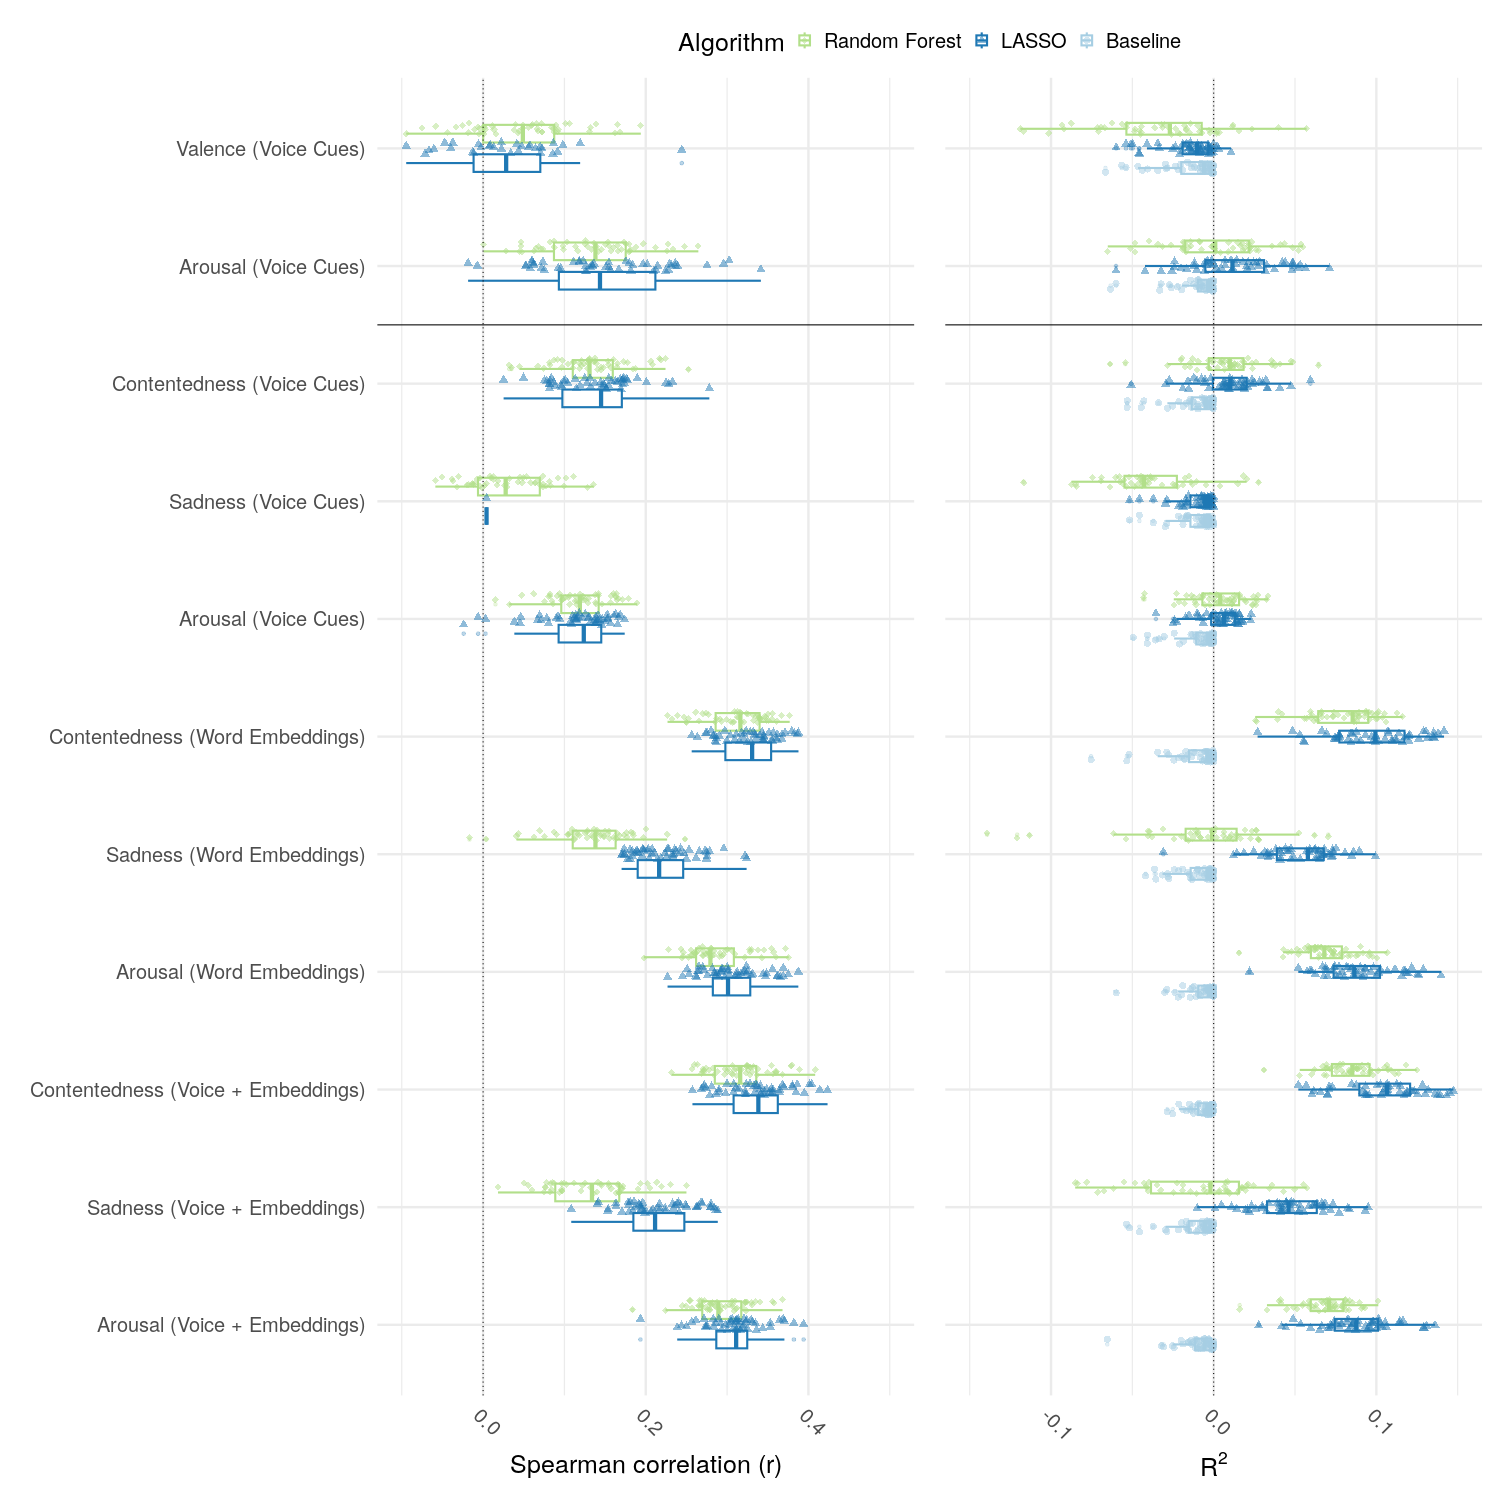
\includegraphics[width=1\linewidth,height=1\textheight]{../figures/bmr_plot} 

}

\caption[Prediction performance]{Box and whisker plot of prediction performance measures from five times repeated 10-fold cross-validation for each affect measure. The top part above the horizontal line belongs to study 1 (*N*$_participants$ = 408, *N*$_samples$ = 9853) and the part below the horizontal line to study 2(*N*$_participants$ = 589, *N*$_samples$~ = 14913).}\label{fig:predictionoverview}
\end{figure}

\hypertarget{content-effects-on-affect-predictions-from-voice}{%
\subsection{Content effects on affect predictions from voice}\label{content-effects-on-affect-predictions-from-voice}}

In study 1, we analyzed if the experimentally altered emotional content (positive/ neutral/ negative) of the predefined sentences that had been read out by participants had an effect on affect predictions from voice acoustics. There were no significant differences in prediction errors across the three sentence conditions for valence (\emph{F}(2,11873) = 0.09,
\emph{p} \textgreater{} .05) and arousal (\emph{F}(2,11873) = 0.39,
\emph{p} \textgreater{} .05) predictions suggesting that sentences' emotional valence did not influence affect predictions from voice acoustics.

In study 2, in order to exploratively investigate the effect of the emotional valence of the spoken content on affect predictions from voice cues, we used the sentiment score (\emph{M} =0.03, \emph{SD} = 0.30) within the interval of {[}-1; 1{]} that had been assigned to each speech transcript by the Google text-to-speech API. Here, we analyzed the correlation of content sentiment with the the absolute prediction errors in the prediction of self-reported momentary arousal, contentedness, and sadness from voice cues using the LASSO algorithm. Result indicate that content sentiment did not have an effect on affect predictions from voice cues: Correlations of content sentiment with absolute predictions errors was not significant for neither contentedness (\emph{r} = 0.01, \emph{p} \textgreater{} .05), sadness (\emph{r} = -0.01, \emph{p} \textgreater{} .05), nor arousal (\emph{r} = 0, \emph{p} \textgreater{} .05). When interpreting those results, one has to keep in mind that overall the predictive performance of the models trained on voice cues was generally limited. We provide additional figures depicting the residuals in the online supplements.

\newpage

\hypertarget{affective-voice-cues}{%
\subsection{Affective voice cues}\label{affective-voice-cues}}

For those models, that yielded better-than-chance predictions overall (i.e., arousal predictions in study 1 and 2 as well as contentedness predictions in study 2), we investigated the most informative features in a LASSO regularized model that had been trained on the full data sets. Figure \ref{fig:lassobetas} provides an overview of selected voice cues and their respective standardized beta regression weights. When interpreting these results, one has to keep in mind that the voice features are often highly correlated, particularly within feature subgroups. Overall, for arousal predictions from scripted speech more voice cues were retained in the LASSO model and those had higher beta coefficients.
For all emotion targets, the variability in the amplitude of the third formant relative to the fundamental frequency was informative.
For arousal predictions, the first Mel-frequency cepstral coefficient (MFCC) for voiced segments describing the overall spectral shape of the voice signal and the Hammarberg Index, reflecting the balance between high and low spectral energy, were informative across the two studies.
Beyond those voice cues, the rate of change in the spectrum over time, emphasizing how quickly spectral characteristics shift, the average loudness of the voice signal, and the the average bandwidth of the first formant for voiced segments contained affective information for contentedness predictions. These observations are in line with descriptive correlations of voice features and self-reported affect experience that are supplied in the online supplements.
Across these features, there is a blend of spectral properties (MFCCs, spectral flux, formant amplitudes, and bandwidths), voice quality indices (Hammarberg Index), and dynamic characteristics (loudness changes). This mix underscores that emotional expression and perception through voice are multifaceted, with both the static qualities of sound and their temporal variations being crucial. The presence of features unique to either arousal or content predictions further illustrates that while some voice features are broadly applicable to emotional expression, others more specifically align with the nuances of emotional intensity (arousal) or the type of emotion conveyed (contentedness).

\begin{figure}

{\centering 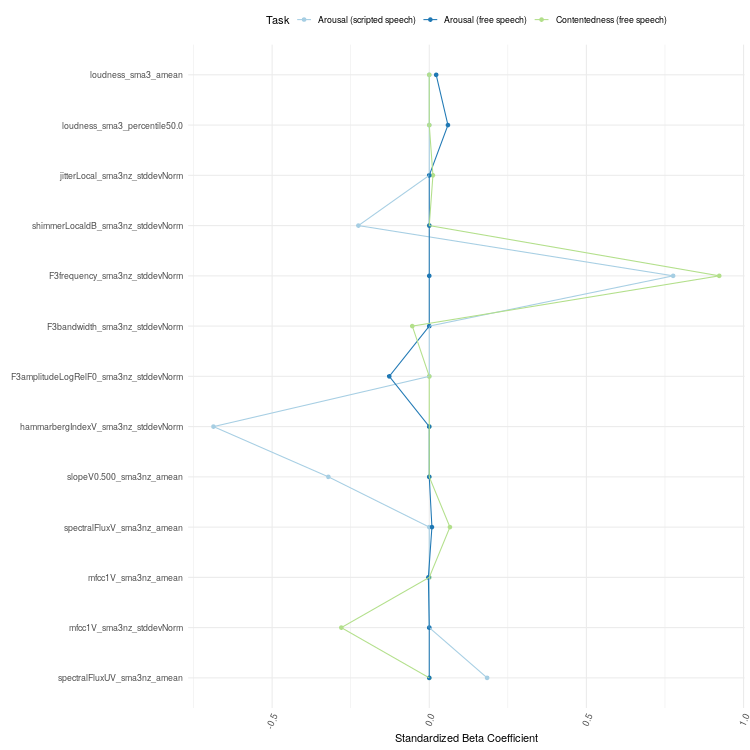
\includegraphics[width=1\linewidth,height=1\textheight]{../figures/betas_plot} 

}

\caption[LASSO betas]{Standardized Beta Coefficients for eGeMAPs voice features from LASSO (Least Absolute Shrinkage and Selection Operator) regularized regression. All voice features that have been selected by any LASSO model for any target variable are shown. The target variables have been standardized to account for their verying scaling in the data sets.}\label{fig:lassobetas}
\end{figure}

\newpage

\hypertarget{discussion}{%
\section{Discussion}\label{discussion}}

In the present work, we extracted acoustic voice parameters and state-of-the-art word embeddings from speech samples collected using smartphones to predict subjective momentary affect experience. In contrast to prior work on the algorithmic recognition of affect expression, our findings suggest that voice cues provide only limited predictive information of subjective affect experience. Here, we identified loudness and features related to fluctuations of the voice spectrum to contain most affective information. Also, experimental (Study 1) and explorative (Study 2) findings suggest that emotional speech content did not affect predictions from voice acoustics (i.e., what someone talks about does not influence how well affect can be predicted from voice cues). Speech content, on the contrary, had been shown to be much more revealing of subjective affect experience.

\hypertarget{voice-contains-little-predictive-information-of-subjective-affect-experience-but-speech-content-does}{%
\subsection{Voice contains little predictive information of subjective affect experience, but speech content does}\label{voice-contains-little-predictive-information-of-subjective-affect-experience-but-speech-content-does}}

Our results indicate that speech samples, and particularly their content, allow for the automatic prediction of subjective momentary affect experience. However, our machine learning models achieve a lower prediction performance as reported in prior work on automatic predictions of affect \emph{expression} (Schuller, 2018). Still, our reported performance is similar to studies predicting subjective affect \emph{experience} from speech samples collected in the wild (Carlier et al., 2022; Sun, Schwartz, Son, Kern, \& Vazire, 2020; Weidman et al., 2020). This observation is in line with prior research suggesting that real-life emotions are more difficult to algorithmically recognize than enacted or elicited emotions (Vogt, André, \& Wagner, 2008). Also, there are only few instances of extreme affect experiences in our data sets compared to the data used in prior studies on acted or labelled emotions. As a result, we rather predicted \emph{mood} in this work, which is, by definition, less intense than emotions (Scherer, 2003) and, consequently, more challenging to recognize.

In Study 2, state-of-the-art word embeddings showed a superior affect prediction performance compared to voice acoustics suggesting that speech content could contain more affective information than speech form. This finding is in line with prior research that found speech content to be more predictive than voice acoustics when predicting momentary subjective experience of happiness (Sun, Schwartz, Son, Kern, \& Vazire, 2020; Weidman et al., 2020). As a consequence, even though prior research has suggested that voice acoustics could be more relevant for human affect inferences than speech content (Ben-David, Multani, Shakuf, Rudzicz, \& van Lieshout, 2016; \textbf{linProsodyDominatesSemantics2020?}), future research and AI applications should consider both channels - content and form - simultaneously.

Furthermore, across the two studies, arousal predictions from voice acoustics were better than those of emotional valence, highlighting prior work showing that the latter is more challenging to automatically infer due to its individual nature (Sridhar \& Busso, 2022). Moreover, in line with prior work (Sun, Schwartz, Son, Kern, \& Vazire, 2020; Weidman et al., 2020), we also ran supplementary analyses for the prediction of within-person fluctuations in affect experience. Overall, those yielded weaker predictions than the between-person differences (see online supplements).

Further, as done in prior research on voice-affect predictions (Weidman et al., 2020), we also compared the prediction performance of machine learning models trained on the much larger Compare2016 (6,737 features) acoustic feature set (Schuller et al., 2016) in contrast to the economic eGeMAPS (88 features) feature set we had used. Just as in prior research, the larger voice feature set did not yield better affect predictions (Weidman et al., 2020). Results are provided in the online supplements. This finding suggests that an economic acoustic feature set is sufficient for affect detection from voice. Moreover, the small features set is less computationally expensive and would allow for online or on-device pre-processing in a scientific or applied setting.

Generally, our findings challenge the transferability of the optimistic prediction results from prior research work on the recognition of affect \emph{expression} (e.g., enacted speech) to the recognition of subjective affect \emph{experience} in everyday speech, particularly from acoustic voice cues. Thereby, our findings also question the proclaimed performance of commercial affect recognition algorithms deployed in daily life that have been mostly trained on enacted or labelled affect \emph{expression}. Consequently, current expectations regarding the performance of emotion-detecting AI services, especially the ones that are focused on voice cues, applied to everyday speech might be overoptimistic. More research is needed to determine how well algorithms can pick up on subjective affect experience from day-to-day speech.

In future research, smartphone could play a prominent role in collecting and analyzing speech data and corresponding in-situ self-reports on subjective affect experience for affect inferences. Hereby, starting from our work, smartphones could be used as a mobile experimental lab to study different aspects of affect recognition from speech, for example by experimentally varying the content as done in Study 1 (Miller, 2012).

\hypertarget{speech-content-has-no-effect-on-affect-predictions-from-voice-cues}{%
\subsection{Speech content has no effect on affect predictions from voice cues}\label{speech-content-has-no-effect-on-affect-predictions-from-voice-cues}}

By experimentally varying the emotional valence of the spoken content in Study 1 and exploratively investigating the effect of word sentiment on voice predictions in Study 2, our findings suggest that the content about what participants talked about did not have a substantial impact on affect predictions from voice cues. This insight could imply that it does not matter what people talk about when algorithmically inferring affect experience from voice cues. However, one has to keep than in mind that affect predictions from voice cues were overall not very strong. More research is needed to disentangle speech content and form in automatic affect recognition.

While the predefined sentences in Study 1 allowed us to control for the emotionality of the content of participants' voice records, they were unable to express themselves freely, which could have impaired predictions from voice acoustics compared to Study 2 where participants could talk freely. As a result, researchers and practitioners should consider the context in which speech had been produced in and keep in mind that findings and trained models might be specific to the given production context and do not necessarily generalize well to other production contexts.

\hypertarget{the-sound-of-emotionaly-prosody-is-complex}{%
\subsection{The sound of emotionaly prosody is complex}\label{the-sound-of-emotionaly-prosody-is-complex}}

Our findings contribute to the literature on voice-affect links. As stated in prior work on affect expressions, voice quality was informative for affective arousal
(Banse \& Scherer, 1996; Larrouy-Maestri, Poeppel, \& Pell, 2024; van Rijn \& Larrouy-Maestri, 2023; Vogt, André, \& Wagner, 2008; Weninger, Eyben, Schuller, Mortillaro, \& Scherer, 2013).

\hypertarget{limitations-and-future-directions}{%
\subsection{Limitations and future directions}\label{limitations-and-future-directions}}

The findings of this work are limited in four ways. First, we used slightly different operationalizations of affect experience and sample compositions in the two studies that might affect their comparability: In Study 1, we assessed valence and arousal on a six-point Likert scale. In Study 2, we used two items to assess affective valence (contentedness and sadness) and arousal on five-/four-point Likert scales. As a consequence, those findings might not be directly comparable. Further, while Study 1 drew on a representative German sample, Study 2 was based on a student convenience sample from the United States with the respective limitations, such as potential constraints in generalizability (Müller, Chen, Peters, Chaintreau, \& Matz, 2021). Also, the German data set that was analyzed in study 1 only contained Android users because of the technical requirements of the logging software. However, past research suggests that the selection bias regarding participant demographics and personality for the German population is negligible (\textbf{schoedelSnapshotsDailyLife2022?}; \textbf{gotzUsersMainSmartphone2017?}; \textbf{keuschCoverageErrorData2020?}). Moreover, both data sets have been collected in western countries, specifically Germany and the United States. Prior research suggests that there are cultural differences in emotion experience (Lim, 2016) and that mood inference models from sensing data do not necessarily generalize to other countries and cultures (\textbf{meegahapolaGeneralizationPersonalizationMobile2023?}). Therefore, future studies should investigate multiple target emotions in diverse international samples from different cultural contexts in non-western countries.

Second, in contrast to prior work using passive speech sensing (e.g., via the EAR), our participants had to actively log their speech in the present work. This artificial setting might have had an effect on results. Moreover, the findings of this study might be subject to the specific instructions that had been given for the audio records. While affect-linked acoustic voice cues in the two studies are similar and are possibly transferable to new voice data, word embeddings are specific to the given task in Study 2. In this manner, future work should employ multiple different speech tasks for affect predictions and investigate how well predictions generalize from one to another.

Also, it should be noted that affective self-reports only from those situations when participants had their smartphone on them and felt comfortable to complete the experience sampling had been analyzed in the present work. Moreover, study participants knew that their affect self-reports and corresponding language samples would be recorded and later analyzed. As a consequence, with regard to assessed subjective affect experience, participants might have only completed the experience sampling questionnaire in selected affective situations, for example not when they were experiencing extreme affective states, or they had not reported on extreme affect at all (\textbf{schoedelSnapshotsDailyLife2022?}). Moreover, participants might have not spoken as naturally as they would if they had not known that their data would be scientifically analyzed. Participants might have made the audio records only in selected suitable situations, for example when they were alone in a quiet place.

Moreover, specifically to Study 1, another related limitation lies in our privacy-preserving on-device data pre-processing approach. By applying on-device feature extraction, we had no opportunity to check in detail if participants truly complied with study instructions and had recorded their voice while reading out the predefined sentences accordingly (beyond the data-driven quality checks we had applied). Further, our approach did not allow to control for records' background noise (e.g., when participants were outside next to a road) or how they held their smartphone during the voice record. However, gender predictions yielded very good prediction results (prediction accuracy = 91.54\%) indicating good data quality. Since checking single raw audio files manually would be out of scope, future research could investigate additional data-driven approaches to check speech data quality directly on the device. Finally, in future work, smartphones could be used to log and immediately pre-process participants' everyday speech by using pre-trained language models to extract content features (e.g., specific topics or word embeddings) directly on the device, too. Thereby, no raw speech data would have to be transferred to a server and valuable information of language's content could be also used for privacy-respectful affect recognition.

Third, the data is comprised of in-situ self-reports of affect experience from participants' everyday life in a non-clinical population. As a result, the data represents the ``normal'' everyday \emph{moods} of regular people with only few cases of extreme affect experience. As a result, the trained affect recognition models should be considered in this context. If the conducted analyses were to be replicated in a clinical sample that contains more cases of extreme affect experience, findings might be more distinct. This does not necessarily mean, however, that findings and prediction models from the present work generalize well to a clinical sample. Alternatively, future studies could aim to collect language samples when participants are known to experience strong emotions, for example based on their physiological signals (\textbf{hoemannContextawareExperienceSampling2020a?}).

Fourth and finally, the ground truth, i.e., the information that is assumed to be fundamentally true, used for model training and evaluation are self-reports on participants' subjective affect experience that are prone to response biases (\textbf{gaoInvestigatingReliabilitySelfreport2021?}). The introduced measurement error can have an impact on predictive modeling (Jacobucci \& Grimm, 2020). Moreover, we employed single items to assess momentary affect experience on different dimensions (i.e., valence and arousal). This is an established approach to reduce participant burden, but can introduce additional measurement error (\textbf{dejonckheereAssessingReliabilitySingleitem2022?}). Therefore, future studies that are particularly interested in subjective affect experience should use multiple items assessing a broad range of affect experience in an intensive longitudinal design. Beyond the psychometric challenges associated with using (single item) self-reports to assess momentary affect experience, there is a conceptual debate on how much of an underlying psychological construct, i.e., of affect experience, one can assess using questionnaires. In order to report one's affect experience most accurately through a survey item, one needs to have introspection to recognize it and have an adequate understanding to communicate it accordingly (\textbf{montagWeStillNeed2022?}; \textbf{boydPersonalityPanoramaConceptualizing2020?}). However, people can vary greatly in that regard (\textbf{critchleyInteroceptionEmotion2017?}). Possibly, in the future, algorithms can replace self-report questionnaires altogether by analyzing natural language directly since transformers (that use word embeddings as employed in study 2) have been reported to approach the upper limits in accuracy already (\textbf{kjellNaturalLanguageAnalyzed2022?}).

\hypertarget{conclusion}{%
\section{Conclusion}\label{conclusion}}

In this work, we investigated if machine learning algorithms can recognize subjective affect experience from speech samples collected in the wild using smartphones. Extracted acoustic voice parameters provided limited predictive information of affective arousal across both studies, while speech content as reflected in state-of-the-art word embeddings had been shown to be predictive of arousal as well emotional valence. Further, experimental and explorative findings suggest that emotional speech content did not affect predictions from voice acoustics (i.e., what someone talked about did not affect how well emotions could be predicted from voice cues). Our findings challenge the transferability of the optimistic prediction results from prior research work and commercial emotion-detection AI algorithms on the recognition of affect \emph{expression} (e.g., enacted and labelled speech) to the recognition of subjective affect \emph{experience} in everyday speech. Finally, we discussed resulting implications for the algorithmic monitoring of affect experience.

\newpage

\hypertarget{references}{%
\section{References}\label{references}}

\hypertarget{refs}{}
\begin{CSLReferences}{1}{0}
\leavevmode\vadjust pre{\hypertarget{ref-banseAcousticProfilesVocal1996}{}}%
Banse, R., \& Scherer, K. R. (1996). Acoustic profiles in vocal emotion expression. \emph{Journal of Personality and Social Psychology}, \emph{70}(3), 614--636. \url{https://doi.org/10.1037/0022-3514.70.3.614}

\leavevmode\vadjust pre{\hypertarget{ref-batlinerAutomaticRecognitionEmotions2011}{}}%
Batliner, A., Schuller, B., Seppi, D., Steidl, S., Devillers, L., Vidrascu, L., \ldots{} Amir, N. (2011). The {Automatic Recognition} of {Emotions} in {Speech}. In \emph{Cognitive {Technologies}} (pp. 71--99). \url{https://doi.org/10.1007/978-3-642-15184-2_6}

\leavevmode\vadjust pre{\hypertarget{ref-banzigerIntroducingGenevaMultimodal2012}{}}%
Bänziger, T., Mortillaro, M., \& Scherer, K. R. (2012). Introducing the {Geneva Multimodal} expression corpus for experimental research on emotion perception. \emph{Emotion (Washington, D.C.)}, \emph{12}(5), 1161--1179. \url{https://doi.org/10.1037/a0025827}

\leavevmode\vadjust pre{\hypertarget{ref-ben-davidProsodySemanticsAre2016}{}}%
Ben-David, B., Multani, N., Shakuf, V., Rudzicz, F., \& van Lieshout, P. H. H. M. (2016). Prosody and {Semantics Are Separate} but {Not Separable Channels} in the {Perception} of {Emotional Speech}: {Test} for {Rating} of {Emotions} in {Speech}. \emph{Journal of Speech, Language, and Hearing Research}, \emph{59}(1), 72--89. \url{https://doi.org/10.1044/2015_JSLHR-H-14-0323}

\leavevmode\vadjust pre{\hypertarget{ref-burkhardtDatabaseGermanEmotional2005a}{}}%
Burkhardt, F., Paeschke, A., Rolfes, M., Sendlmeier, W., \& Weiss, B. (2005). A database of {German} emotional speech. In \emph{9th European Conference on Speech Communication and Technology} (Vol. 5, p. 1520). \url{https://doi.org/10.21437/Interspeech.2005-446}

\leavevmode\vadjust pre{\hypertarget{ref-carlierSearchStateTrait2022}{}}%
Carlier, C., Niemeijer, K., Mestdagh, M., Bauwens, M., Vanbrabant, P., Geurts, L., \ldots{} Kuppens, P. (2022). In {Search} of {State} and {Trait Emotion Markers} in {Mobile-Sensed Language}: {Field Study}. \emph{JMIR Mental Health}, \emph{9}(2), e31724. \url{https://doi.org/10.2196/31724}

\leavevmode\vadjust pre{\hypertarget{ref-defrenEmotionalSpeechPerception2018}{}}%
Defren, S., de Brito Castilho Wesseling, P., Allen, S., Shakuf, V., Ben-David, B., \& Lachmann, T. (2018). Emotional {Speech Perception}: {A} set of semantically validated {German} neutral and emotionally affective sentences. \emph{9th {International Conference} on {Speech Prosody} 2018}, 714--718. ISCA. \url{https://doi.org/10.21437/SpeechProsody.2018-145}

\leavevmode\vadjust pre{\hypertarget{ref-eybenGenevaMinimalisticAcoustic2016}{}}%
Eyben, F., Scherer, K. R., Schuller, B. W., Sundberg, J., Andre, E., Busso, C., \ldots{} Truong, K. P. (2016). The {Geneva Minimalistic Acoustic Parameter Set} ({GeMAPS}) for {Voice Research} and {Affective Computing}. \emph{IEEE Transactions on Affective Computing}, \emph{7}(2), 190--202. \url{https://doi.org/10.1109/TAFFC.2015.2457417}

\leavevmode\vadjust pre{\hypertarget{ref-eybenOpensmileMunichVersatile2010}{}}%
Eyben, F., Wöllmer, M., \& Schuller, B. (2010). Opensmile: The munich versatile and fast open-source audio feature extractor. \emph{Proceedings of the International Conference on {Multimedia} - {MM} '10}, 1459. Firenze, Italy: ACM Press. \url{https://doi.org/10.1145/1873951.1874246}

\leavevmode\vadjust pre{\hypertarget{ref-grimmVeraAmMittag2008}{}}%
Grimm, M., Kroschel, K., \& Narayanan, S. (2008). The {Vera} am {Mittag German} audio-visual emotional speech database. \emph{2008 {IEEE International Conference} on {Multimedia} and {Expo}}, 865--868. \url{https://doi.org/10.1109/ICME.2008.4607572}

\leavevmode\vadjust pre{\hypertarget{ref-grossRevealingFeelingsFacets1997}{}}%
Gross, J. A. J., \& John, O. L. I. E. (1997). Revealing feelings: {Facets} of emotional expressivity in self-reports, peer ratings, and expressive behavior. \emph{Journal of Personality and Social Psychology}, 434--447.

\leavevmode\vadjust pre{\hypertarget{ref-grossDissociationEmotionExpression2000}{}}%
Gross, J. J., John, O. P., \& Richards, J. M. (2000). The {Dissociation} of {Emotion Expression} from {Emotion Experience}: {A Personality Perspective}. \emph{Personality and Social Psychology Bulletin}, \emph{26}(6), 712--726. \url{https://doi.org/10.1177/0146167200268006}

\leavevmode\vadjust pre{\hypertarget{ref-hildebrandVoiceAnalyticsBusiness2020}{}}%
Hildebrand, C., Efthymiou, F., Busquet, F., Hampton, W. H., Hoffman, D. L., \& Novak, T. P. (2020). Voice analytics in business research: {Conceptual} foundations, acoustic feature extraction, and applications. \emph{Journal of Business Research}, \emph{121}, 364--374. \url{https://doi.org/10.1016/j.jbusres.2020.09.020}

\leavevmode\vadjust pre{\hypertarget{ref-huangPredictionEmotionChange2018}{}}%
Huang, Z., \& Epps, J. (2018). Prediction of {Emotion Change From Speech}. \emph{Frontiers in ICT}, \emph{5}.

\leavevmode\vadjust pre{\hypertarget{ref-jacobucciMachineLearningPsychological2020}{}}%
Jacobucci, R., \& Grimm, K. J. (2020). Machine {Learning} and {Psychological Research}: {The Unexplored Effect} of {Measurement}. \emph{Perspectives on Psychological Science}, \emph{15}(3), 809--816. \url{https://doi.org/10.1177/1745691620902467}

\leavevmode\vadjust pre{\hypertarget{ref-kjellTextRpackageAnalyzing2021}{}}%
Kjell, O., Giorgi, S., \& Schwartz, H. A. (2021). \emph{Text: {An R-package} for {Analyzing} and {Visualizing Human Language Using Natural Language Processing} and {Deep Learning}}. PsyArXiv. \url{https://doi.org/10.31234/osf.io/293kt}

\leavevmode\vadjust pre{\hypertarget{ref-knightAmazonWorkingMaking2016}{}}%
Knight, W. (2016). Amazon {Working} on {Making Alexa Recognize Your Emotions}. https://www.technologyreview.com/2016/06/13/159665/amazon-working-on-making-alexa-recognize-your-emotions/.

\leavevmode\vadjust pre{\hypertarget{ref-kochPredictingAffectiveStates2021}{}}%
Koch, T., \& Schoedel, R. (2021). \emph{Predicting {Affective States} from {Acoustic Voice Cues Collected} with {Smartphones}}. \url{https://doi.org/10.23668/psycharchives.4454}

\leavevmode\vadjust pre{\hypertarget{ref-langMlr3ModernObjectoriented2019}{}}%
Lang, M., Binder, M., Richter, J., Schratz, P., Pfisterer, F., Coors, S., \ldots{} Bischl, B. (2019). Mlr3: {A} modern object-oriented machine learning framework in {R}. \emph{Journal of Open Source Software}, \emph{4}(44), 1903. \url{https://doi.org/10.21105/joss.01903}

\leavevmode\vadjust pre{\hypertarget{ref-larrouy-maestriSoundEmotionalProsody2024}{}}%
Larrouy-Maestri, P., Poeppel, D., \& Pell, M. D. (2024). The {Sound} of {Emotional Prosody}: {Nearly} 3 {Decades} of {Research} and {Future Directions}. \emph{Perspectives on Psychological Science}, 17456916231217722. \url{https://doi.org/10.1177/17456916231217722}

\leavevmode\vadjust pre{\hypertarget{ref-limCulturalDifferencesEmotion2016}{}}%
Lim, N. (2016). Cultural differences in emotion: Differences in emotional arousal level between the {East} and the {West}. \emph{Integrative Medicine Research}, \emph{5}(2), 105--109. \url{https://doi.org/10.1016/j.imr.2016.03.004}

\leavevmode\vadjust pre{\hypertarget{ref-liuRoBERTaRobustlyOptimized2019}{}}%
Liu, Y., Ott, M., Goyal, N., Du, J., Joshi, M., Chen, D., \ldots{} Stoyanov, V. (2019). \emph{{RoBERTa}: {A Robustly Optimized BERT Pretraining Approach}}. arXiv. \url{https://doi.org/10.48550/arXiv.1907.11692}

\leavevmode\vadjust pre{\hypertarget{ref-mandellSpotifyPatentsVoice2020}{}}%
Mandell, J. (2020). Spotify {Patents A Voice Assistant That Can Read Your Emotions}. https://www.forbes.com/sites/joshmandell/2020/03/12/spotify-patents-a-voice-assistant--that-can-read-your-emotions/.

\leavevmode\vadjust pre{\hypertarget{ref-marreroEvaluatingVoiceSamples2022}{}}%
Marrero, Z. N. K., Gosling, S. D., Pennebaker, J. W., \& Harari, G. M. (2022). Evaluating voice samples as a potential source of information about personality. \emph{Acta Psychologica}, \emph{230}, 103740. \url{https://doi.org/10.1016/j.actpsy.2022.103740}

\leavevmode\vadjust pre{\hypertarget{ref-materoEvaluatingContextualEmbeddings2022}{}}%
Matero, M., Hung, A., \& Schwartz, H. A. (2022). Evaluating {Contextual Embeddings} and their {Extraction Layers} for {Depression Assessment}. \emph{Proceedings of the 12th {Workshop} on {Computational Approaches} to {Subjectivity}, {Sentiment} \& {Social Media Analysis}}, 89--94. Dublin, Ireland: Association for Computational Linguistics. \url{https://doi.org/10.18653/v1/2022.wassa-1.9}

\leavevmode\vadjust pre{\hypertarget{ref-mehlElectronicallyActivatedRecorder2017}{}}%
Mehl, M. R. (2017). The {Electronically Activated Recorder} ({EAR}): {A Method} for the {Naturalistic Observation} of {Daily Social Behavior}. \emph{Current Directions in Psychological Science}, \emph{26}(2), 184--190. \url{https://doi.org/10.1177/0963721416680611}

\leavevmode\vadjust pre{\hypertarget{ref-millerSmartphonePsychologyManifesto2012}{}}%
Miller, G. (2012). The {Smartphone Psychology Manifesto}. \emph{Perspectives on Psychological Science: A Journal of the Association for Psychological Science}, \emph{7}(3), 221--237. \url{https://doi.org/10.1177/1745691612441215}

\leavevmode\vadjust pre{\hypertarget{ref-millingSpeechNewBlood2022}{}}%
Milling, M., Pokorny, F., Bartl-Pokorny, K., \& Schuller, B. (2022). Is {Speech} the {New Blood}? {Recent Progress} in {AI-Based Disease Detection From Audio} in a {Nutshell}. \emph{Frontiers in Digital Health}, \emph{4}, 886615. \url{https://doi.org/10.3389/fdgth.2022.886615}

\leavevmode\vadjust pre{\hypertarget{ref-mullerDepressionPredictionsGPSbased2021}{}}%
Müller, S. R., Chen, X. L., Peters, H., Chaintreau, A., \& Matz, S. C. (2021). Depression predictions from {GPS-based} mobility do not generalize well to large demographically heterogeneous samples. \emph{Scientific Reports}, \emph{11}(1), 14007. \url{https://doi.org/10.1038/s41598-021-93087-x}

\leavevmode\vadjust pre{\hypertarget{ref-schererVocalCommunicationEmotion2003}{}}%
Scherer, K. (2003). Vocal communication of emotion: {A} review of research paradigms. \emph{Speech Communication}, \emph{40}(1-2), 227--256. \url{https://doi.org/10.1016/S0167-6393(02)00084-5}

\leavevmode\vadjust pre{\hypertarget{ref-schoedelBasicProtocolSmartphone2020}{}}%
Schoedel, R., \& Oldemeier, M. (2020). \emph{Basic {Protocol}: {Smartphone Sensing Panel Study}}. \url{https://doi.org/10.23668/psycharchives.2901}

\leavevmode\vadjust pre{\hypertarget{ref-schullerSpeechEmotionRecognition2018}{}}%
Schuller, B. (2018). Speech emotion recognition: Two decades in a nutshell, benchmarks, and ongoing trends. \emph{Communications of the ACM}, \emph{61}(5), 90--99. \url{https://doi.org/10.1145/3129340}

\leavevmode\vadjust pre{\hypertarget{ref-schullerINTERSPEECH2016Computational2016}{}}%
Schuller, B., Steidl, S., Batliner, A., Hirschberg, J., Burgoon, J., Baird, A., \ldots{} Evanini, K. (2016). \emph{The {INTERSPEECH} 2016 {Computational Paralinguistics Challenge}: {Deception}, {Sincerity} and {Native Language}} (p. 2005). \url{https://doi.org/10.21437/Interspeech.2016-129}

\leavevmode\vadjust pre{\hypertarget{ref-schwartzEmotionalSpeechProcessing2012}{}}%
Schwartz, R., \& Pell, M. D. (2012). Emotional {Speech Processing} at the {Intersection} of {Prosody} and {Semantics}. \emph{PLoS ONE}, \emph{7}(10), e47279. \url{https://doi.org/10.1371/journal.pone.0047279}

\leavevmode\vadjust pre{\hypertarget{ref-sridharUnsupervisedPersonalizationEmotion2022}{}}%
Sridhar, K., \& Busso, C. (2022). Unsupervised {Personalization} of an {Emotion Recognition System}: {The Unique Properties} of the {Externalization} of {Valence} in {Speech}. \emph{IEEE Transactions on Affective Computing}, \emph{13}(4), 1959--1972. \url{https://doi.org/10.1109/TAFFC.2022.3187336}

\leavevmode\vadjust pre{\hypertarget{ref-sunLanguageWellbeingTracking2020}{}}%
Sun, J., Schwartz, H. A., Son, Y., Kern, M. L., \& Vazire, S. (2020). The language of well-being: {Tracking} fluctuations in emotion experience through everyday speech. \emph{Journal of Personality and Social Psychology}, \emph{118}(2), 364--387. \url{https://doi.org/10.1037/pspp0000244}

\leavevmode\vadjust pre{\hypertarget{ref-vanrijnModellingIndividualCrosscultural2023}{}}%
van Rijn, P., \& Larrouy-Maestri, P. (2023). Modelling individual and cross-cultural variation in the mapping of emotions to speech prosody. \emph{Nature Human Behaviour}, \emph{7}(3), 386--396. \url{https://doi.org/10.1038/s41562-022-01505-5}

\leavevmode\vadjust pre{\hypertarget{ref-vlahosTalkMeHow2019}{}}%
Vlahos, J. (2019). \emph{Talk to {Me}: {How Voice Computing Will Transform} the {Way We Live}, {Work}, and {Think}}. Eamon Dolan Books.

\leavevmode\vadjust pre{\hypertarget{ref-vogtAutomaticRecognitionEmotions2008}{}}%
Vogt, T., André, E., \& Wagner, J. (2008). Automatic {Recognition} of {Emotions} from {Speech}: {A Review} of the {Literature} and {Recommendations} for {Practical Realisation}. In C. Peter \& R. Beale (Eds.), \emph{Affect and {Emotion} in {Human-Computer Interaction}} (Vol. 4868, pp. 75--91). Berlin, Heidelberg: Springer Berlin Heidelberg. \url{https://doi.org/10.1007/978-3-540-85099-1_7}

\leavevmode\vadjust pre{\hypertarget{ref-weidmanNotHearingHappiness2020}{}}%
Weidman, A. C., Sun, J., Vazire, S., Quoidbach, J., Ungar, L. H., \& Dunn, E. W. (2020). ({Not}) hearing happiness: {Predicting} fluctuations in happy mood from acoustic cues using machine learning. \emph{Emotion (Washington, D.C.)}, \emph{20}(4), 642--658. \url{https://doi.org/10.1037/emo0000571}

\leavevmode\vadjust pre{\hypertarget{ref-weningerAcousticsEmotionAudio2013}{}}%
Weninger, F., Eyben, F., Schuller, B. W., Mortillaro, M., \& Scherer, K. R. (2013). On the {Acoustics} of {Emotion} in {Audio}: {What Speech}, {Music}, and {Sound} have in {Common}. \emph{Frontiers in Psychology}, \emph{4}. \url{https://doi.org/10.3389/fpsyg.2013.00292}

\leavevmode\vadjust pre{\hypertarget{ref-wiltingRealVsActed2006}{}}%
Wilting, J., Krahmer, E. J., \& Swerts, M. G. J. (2006). Real vs. Acted emotional speech. \emph{Proceedings of the International Conference on Spoken Language Processing (Interspeech 2006)}.

\leavevmode\vadjust pre{\hypertarget{ref-wrightRangerFastImplementation2017}{}}%
Wright, M. N., \& Ziegler, A. (2017). Ranger: {A Fast Implementation} of {Random Forests} for {High Dimensional Data} in {C}++ and {R}. \emph{Journal of Statistical Software}, \emph{77}(1), 1--17. \url{https://doi.org/10.18637/jss.v077.i01}

\leavevmode\vadjust pre{\hypertarget{ref-wuMultimodalDataCollection2021}{}}%
Wu, C., Fritz, H., Bastami, S., Maestre, J. P., Thomaz, E., Julien, C., \ldots{} Nagy, Z. (2021). Multi-modal data collection for measuring health, behavior, and living environment of large-scale participant cohorts. \emph{GigaScience}, \emph{10}(6). \url{https://doi.org/10.1093/gigascience/giab044}

\end{CSLReferences}


\end{document}
